\section{PlantVillage Dataset}

    \subsection{Overview}
    PlantVillage is a dataset consisting of 54303 healthy and unhealthy leaf images divided into 38 classes by species and disease.
    \begin{figure}
        \centering
        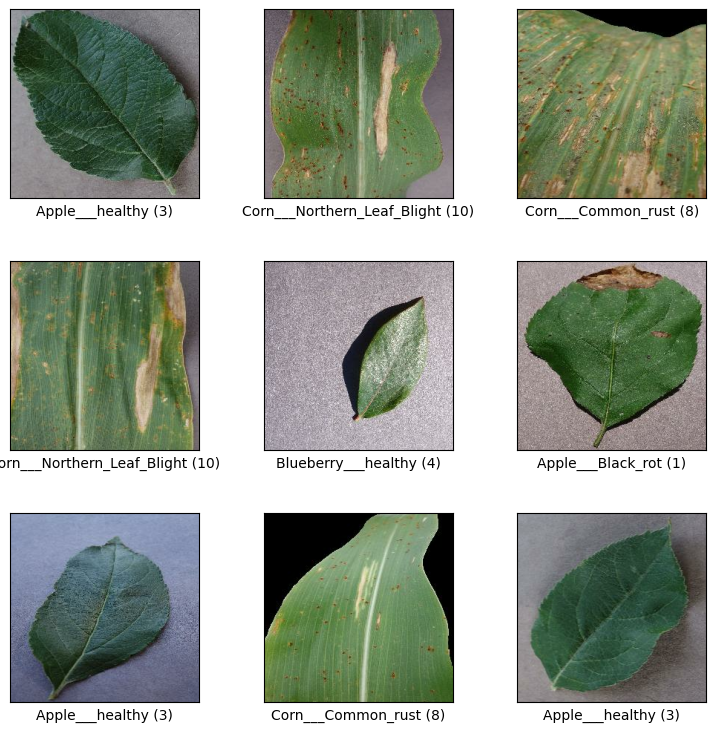
\includegraphics[width=\linewidth]{graphics//chapter 4/plant village dataset viz.png}
        \caption{Plant Village Datasets}
        \label{fig:plant village vizl}
    \end{figure}
    
    \subsection{Original classes and labels}
        It consists of the following 38 classes and has a total of 54303 items.

    \begin{figure}
        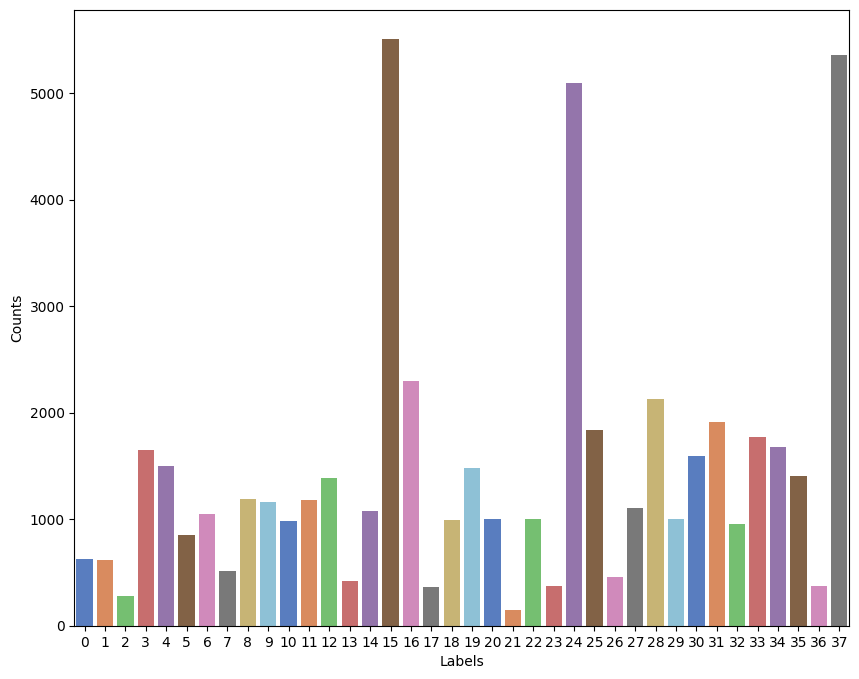
\includegraphics[width=1\linewidth]{graphics//chapter 4/38 class distribution.png}
        \caption{Class Distribution Before Class Reduction}
        \label{Class Distribution Before Class Reduction}
    \end{figure}

    
    \begin{multicols}{2}
    \begin{enumerate}
    \item Apple\_scab
    \item Apple\_black\_rot
    \item Apple\_cedar\_apple\_rust
    \item Apple\_healthy
    \item Background\_without\_leaves
    \item Blueberry\_healthy
    \item Cherry\_powdery\_mildew
    \item Cherry\_healthy
    \item Corn\_gray\_leaf\_spot
    \item Corn\_common\_rust
    \item Corn\_northern\_leaf\_blight
    \item Corn\_healthy
    \item Grape\_black\_rot
    \item Grape\_black\_measles
    \item Grape\_leaf\_blight
    \item Grape\_healthy
    \item Orange\_haunglongbing
    \item Peach\_bacterial\_spot
    \item Peach\_healthy
    \item Pepper\_bacterial\_spot
    \item Pepper\_healthy
    \item Potato\_early\_blight
    \item Potato\_healthy
    \item Potato\_late\_blight
    \item Raspberry\_healthy
    \item Soybean\_healthy
    \item Squash\_powdery\_mildew
    \item Strawberry\_healthy
    \item Strawberry\_leaf\_scorch
    \item Tomato\_bacterial\_spot
    \item Tomato\_early\_blight
    \item Tomato\_healthy
    \item Tomato\_late\_blight
    \item Tomato\_leaf\_mold
    \item Tomato\_septoria\_leaf\_spot
    \item Tomato\_spider\_mites\_two-spotted\_spider\_mite
    \item Tomato\_target\_spot
    \item Tomato\_mosaic\_virus
    \item Tomato\_yellow\_leaf\_curl\_virus
    \end{enumerate}
    \end{multicols}

    \vspace{1em}

    \subsection{Classes used}
    We have narrowed down these 38 classes to 11 classes, because of hardware constraints.\par \vspace{1em}

    
    
    The narrowed-down classes, totaling 10431 items are:

    \begin{multicols}{2}
    \begin{enumerate}
    \item Apple\_Apple\_scab
    \item Apple\_Black\_rot
    \item Apple\_Cedar\_apple\_rust
    \item Apple\_healthy
    \item Blueberry\_healthy
    \item Cherry\_healthy
    \item Cherry\_Powdery\_mildew
    \item Corn\_Cercospora\_leaf\_spot\_Gray\_leaf\_spot
    \item Corn\_Common\_rust
    \item Corn\_healthy
    \item Corn\_Northern\_Leaf\_Blight
    \end{enumerate}
    \end{multicols}

    \subsection{Item Data Composition}
    The original PlantVillage data was mildly imbalanced as such, our dataset also suffers from mild data imbalance.

    \begin{figure}
        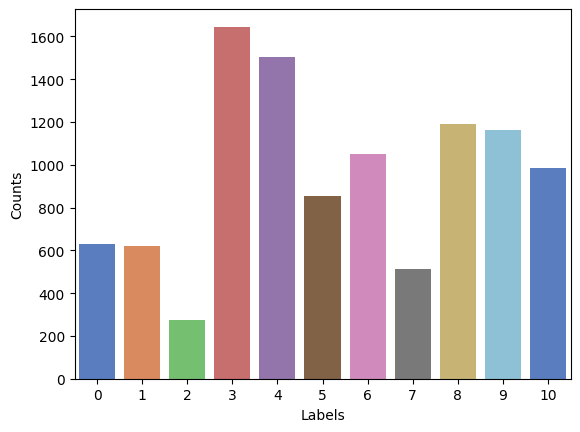
\includegraphics[width=0.8\textwidth, center]{graphics/chapter 4/Image_Classifications.png}
        \caption{Class distribution after class reduction}
    \end{figure}
     \par \vspace{1em}
     
    Key:
    \begin{multicols}{2}
    \begin{enumerate}
        \setcounter{enumi}{-1}
        \item Apple\_Apple\_scab
        \item Apple\_Black\_rot
        \item Apple\_Cedar\_apple\_rust
        \item Apple\_healthy
        \item Blueberry\_healthy
        \item Cherry\_healthy
        \item Cherry\_Powdery\_mildew
        \item Corn\_Cercospora\_leaf\_spot\_Gray\_leaf\_spot
        \item Corn\_Common\_rust
        \item Corn\_healthy
        \item Corn\_Northern\_Leaf\_Blight
    \end{enumerate}
    \end{multicols}

    \vspace{2em}

    A potential solution to imbalanced classes is to use either:
    \begin{enumerate}
        \item Downsampling (in this context) means training on a disproportionately low subset of the majority class examples.
        \item Upweighting means adding an example weight to the downsampled class equal to the factor by which you downsampled
    \end{enumerate}

    

    

    
    % \item Classes and labels - List of Plant Species and Associated Diseases, 36 11
    
    % \item Number of Classes (11 in total)
    
    % \item Data Composition - Number of Images per Class, Image Resolutions and Formats, Distribution of Images across Classes
    % \item Example Images - Visual Examples of Images from Different Classes,
    %% \item Variability in Image Quality and Conditions


\par

\newpage